\documentclass{beamer}
\usepackage[french]{babel}
\usepackage[T1]{fontenc}
\usepackage[utf8]{inputenc}
\usepackage{tikz}
\usepackage{graphicx}
\usetheme{Warsaw}
\setbeamertemplate{page number in head/foot}[totalframenumber]
\usepackage{hyperref}
\title{Interpréteur de Système de Lindenmayer}
\author{Boubacar Sadio DIALLO \and Damien MARIS \and Evens ANTOINE \and Manix-Emmanuel BIDUAYA MBUYI}
\date{Mercredi 03 Mai 2023}


\begin{document}
\frame{\titlepage}

\begin{frame}{Introduction \& Plan }
    \tableofcontents
\end{frame}
\section{Aperçu du produit final}
\begin{frame}{Aperçu de notre produit final}
    \begin{figure}[h]
	   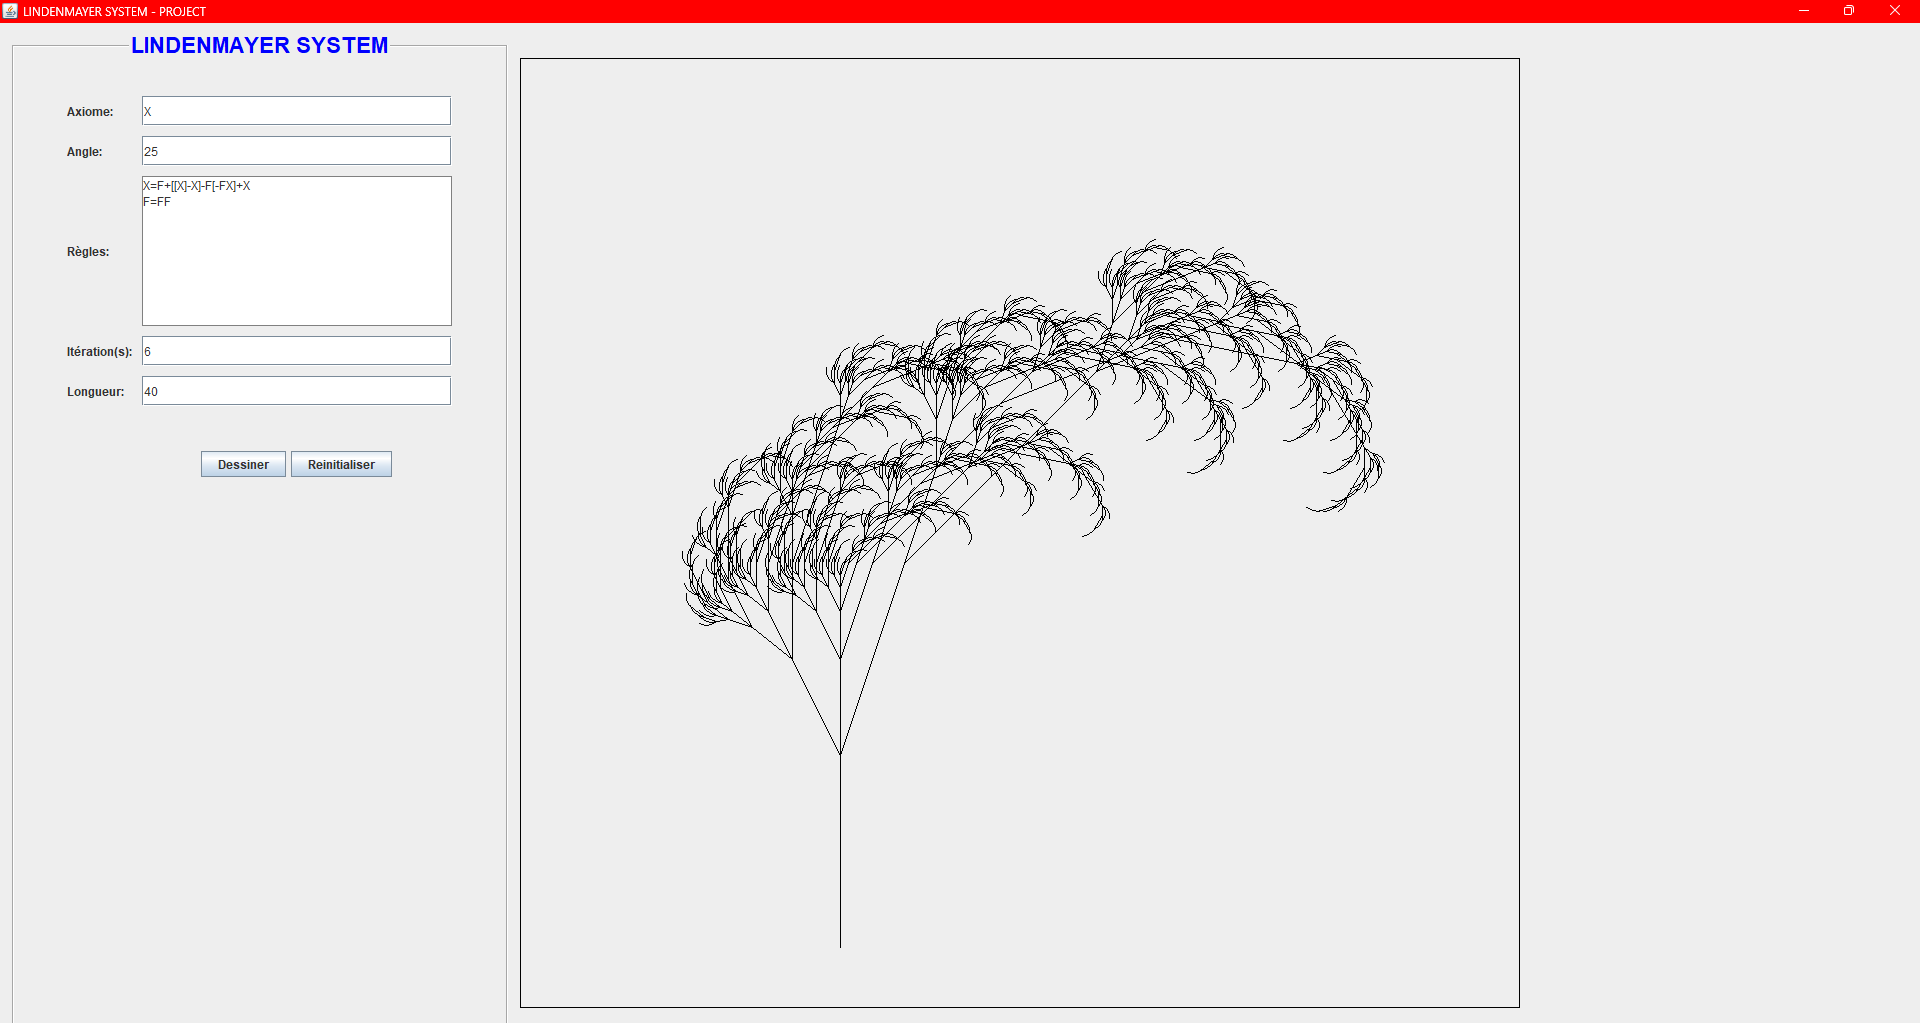
\includegraphics[width=\textwidth]{./images/ArbreFractal.png}
	   \caption{Interpréteur L-System (exemple)}
    \end{figure}
\end{frame}

\section{Conception}
\begin{frame}{Conception}
     Comment avons-nous choisi de programmer notre interpréteur de L-Système ?
     \begin{enumerate}
         \item L'alphabet
         \item La tortue
         \item Le L-Système
         \item L'interface graphique
     \end{enumerate}
\end{frame}
\subsection{Alphabétisation}

\subsubsection{Notre alphabet}
\begin{frame}{Notre alphabet}
    \begin{itemize}
        \item Présentation de l'alphabet d'un L-Système
        \item Fonctionnement de notre alphabet
        \item La classe mère Symbole
    \end{itemize}
\end{frame}
\subsubsection{Ses classes dérivées}
\begin{frame}{Ses classes dérivées}
Les classes dérivantes de Symbole :
    \begin{columns}[T]
        \begin{column}{0.5\textwidth}
            \begin{itemize}
            	\item DessinerAvancer : \textbf{F}
            	\item Avancer : \textbf{f}
            	\item TournerSensHoraire : \textbf{-}
            	\item TournerSensTrigo : \textbf{+} 
            	\item SauverPosition : \textbf{[} 
            	\item RestaurerPosition : \textbf{]} 
            \end{itemize}
        \end{column}
        \begin{column}{0.5\textwidth}
            \begin{itemize}
            	\item DemiTour : \textbf{|} 
            	\item Nord : \textbf{\^}
            	\item Sud : \textbf{\&} 
            	\item Ouest : \textbf{<}
            	\item Est : \textbf{>}
            \end{itemize}
        \end{column}
    \end{columns}
\end{frame}
\begin{frame}{Alphabet}
    \begin{figure}[h]
	   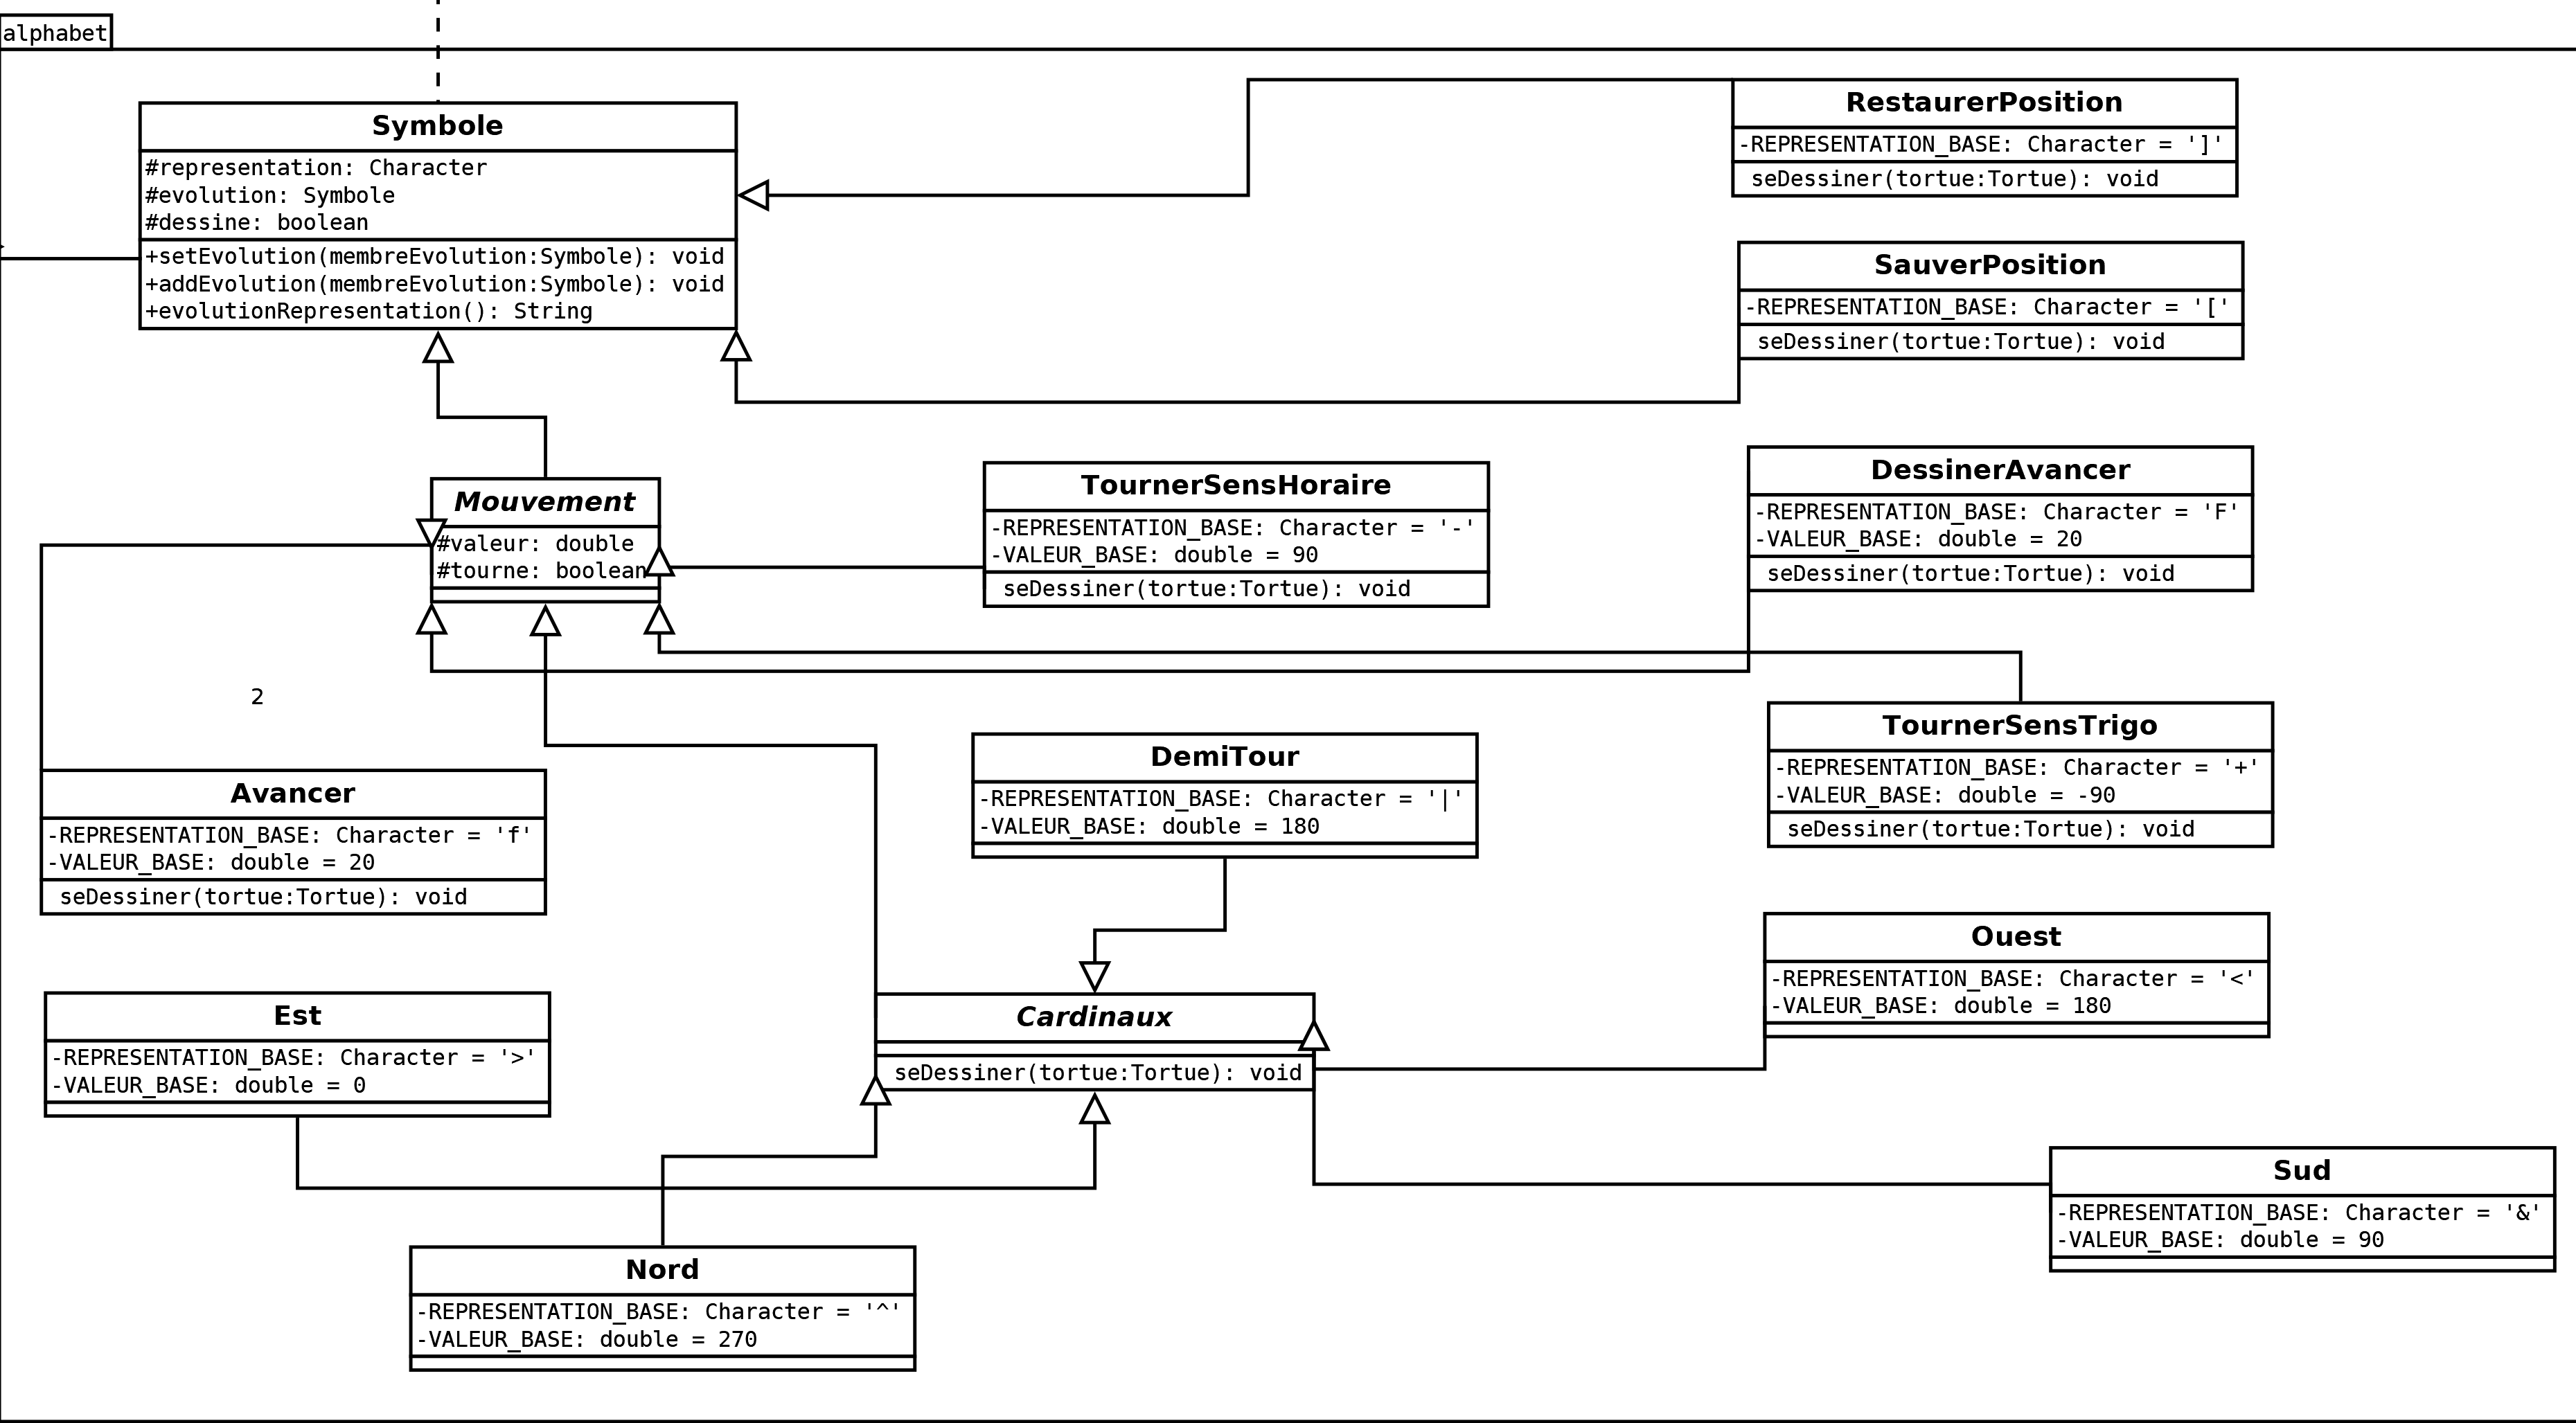
\includegraphics[width=\textwidth]{./images/DiagrammeAlphabet.png}
	   \caption{Diagramme package Alphabet}
    \end{figure}
\end{frame}


\subsection{Tortue}

\begin{frame}{La classe Tortue}
    \begin{itemize}
        \item A quoi sert une tortue?
        \begin{figure}[h]
            \centering
           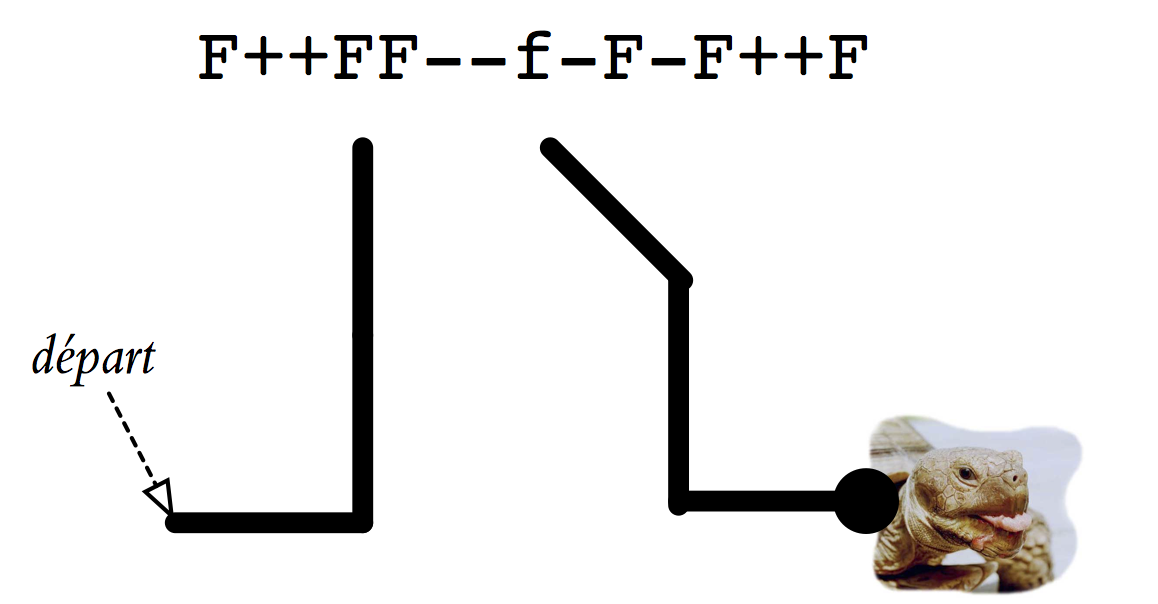
\includegraphics[width=0.5\textwidth]{./images/turtle-graphics.png}
           \caption{Illustration de tortue}
        \end{figure}
        \item Notre tortue, notre choix d'implémentation.
    \end{itemize}
\end{frame}
\begin{frame}{Package tortue}
    \begin{figure}[h]
	   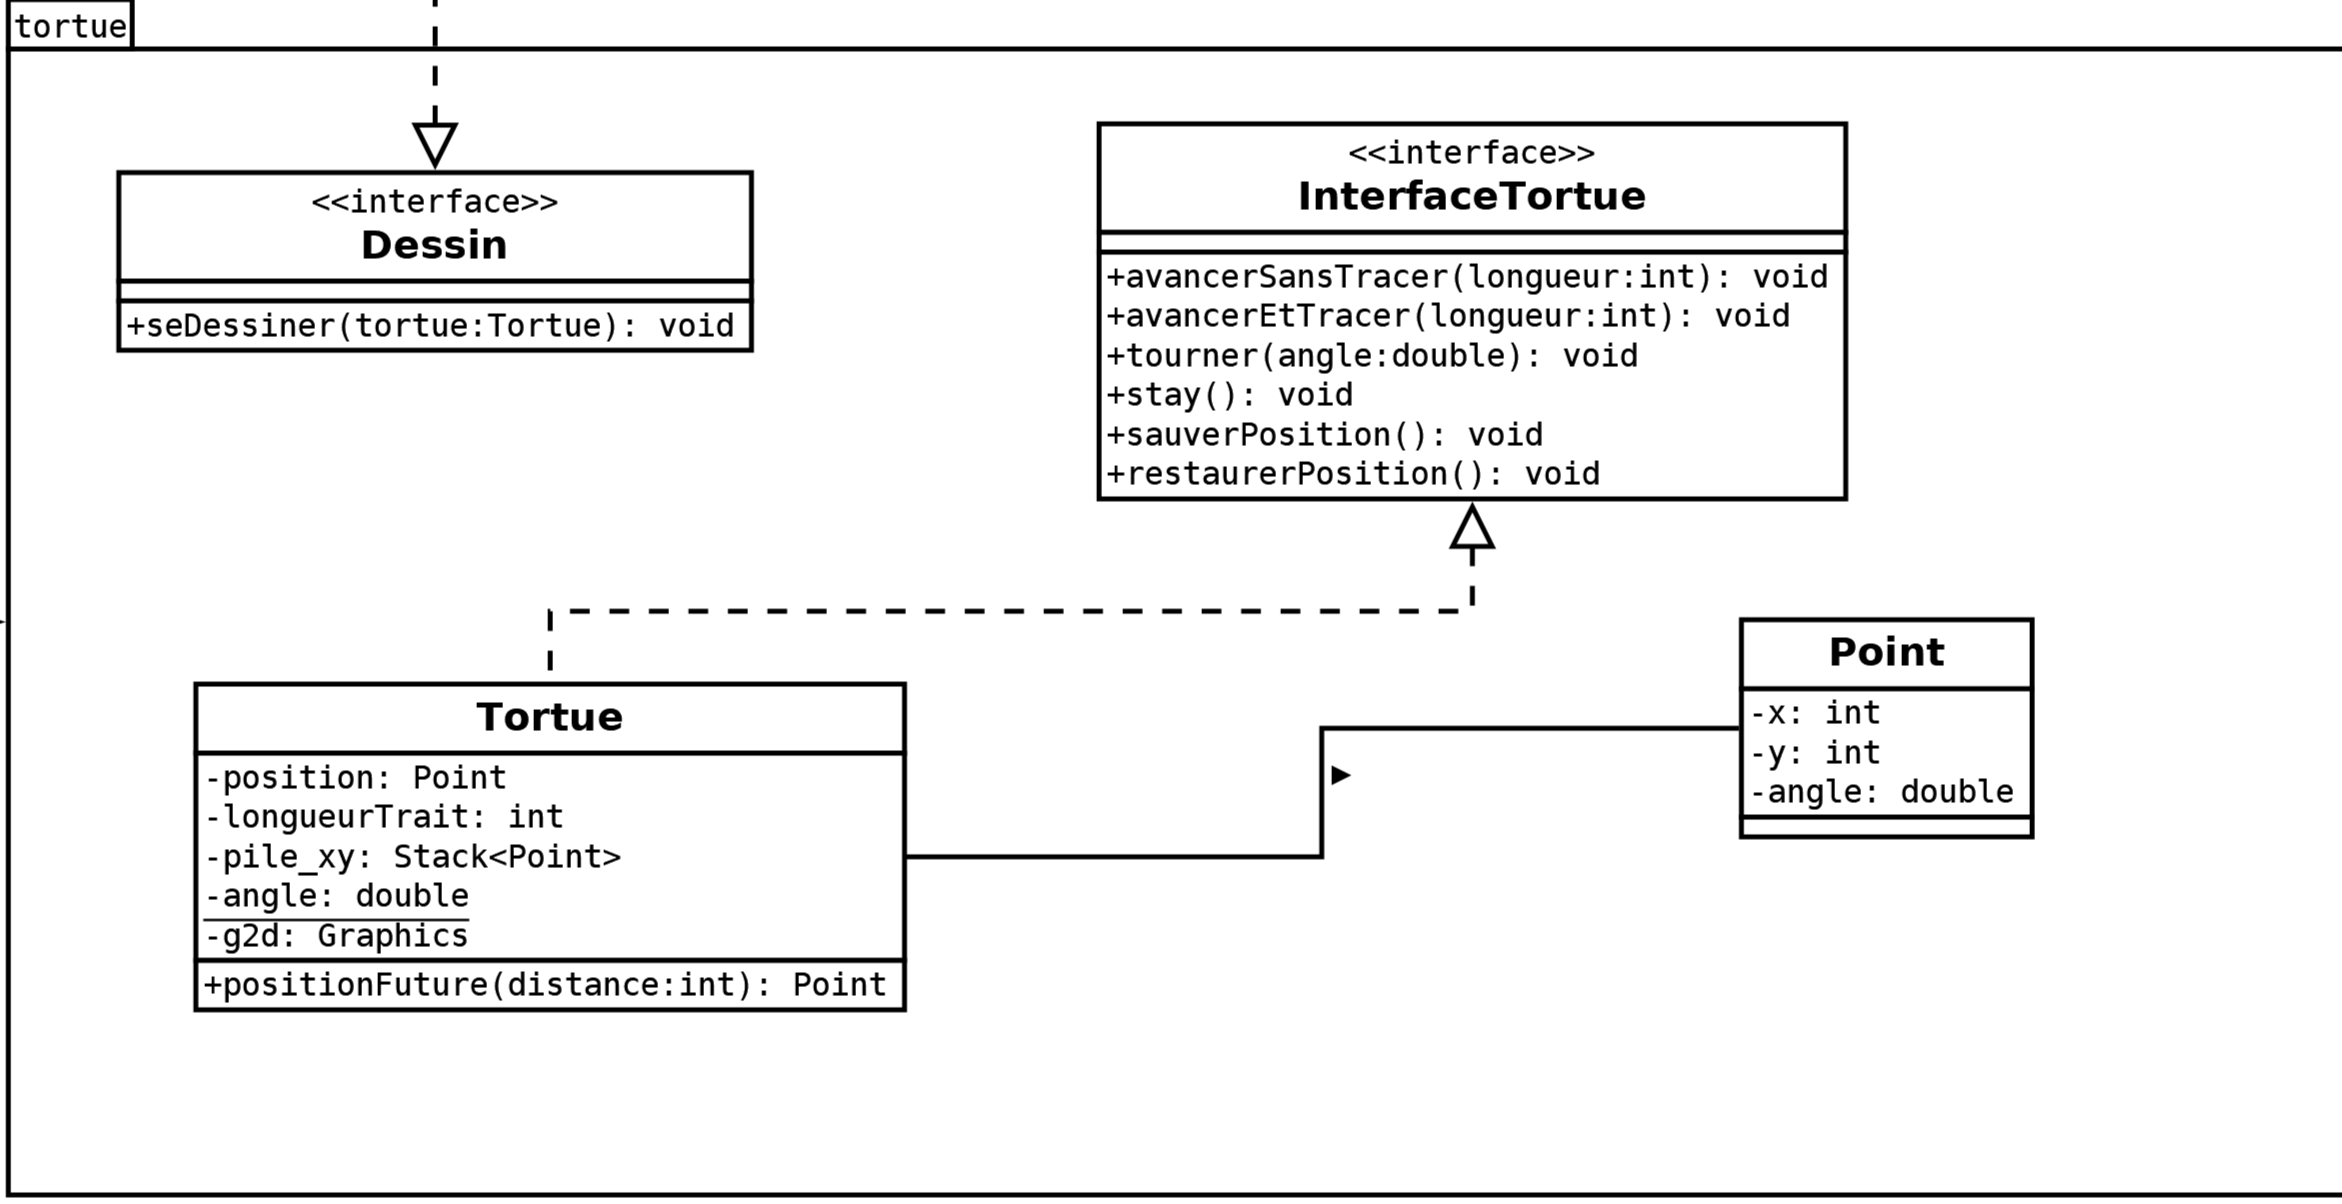
\includegraphics[width=\textwidth]{./images/DiagrammeTortue.png}
	   \caption{Diagramme package Tortue}
    \end{figure}
\end{frame}
\subsection{La classe L-Système}
\begin{frame}{La classe L-Système}
    \begin{columns}
    \begin{column}{0.5\textwidth}
    \begin{itemize}
        \item Ce que représente la classe LSystem
        \item Choix d'implémentation et explications
    \end{itemize}
    \end{column}
    \begin{column}{0.5\textwidth}
    \begin{figure}
        \centering
        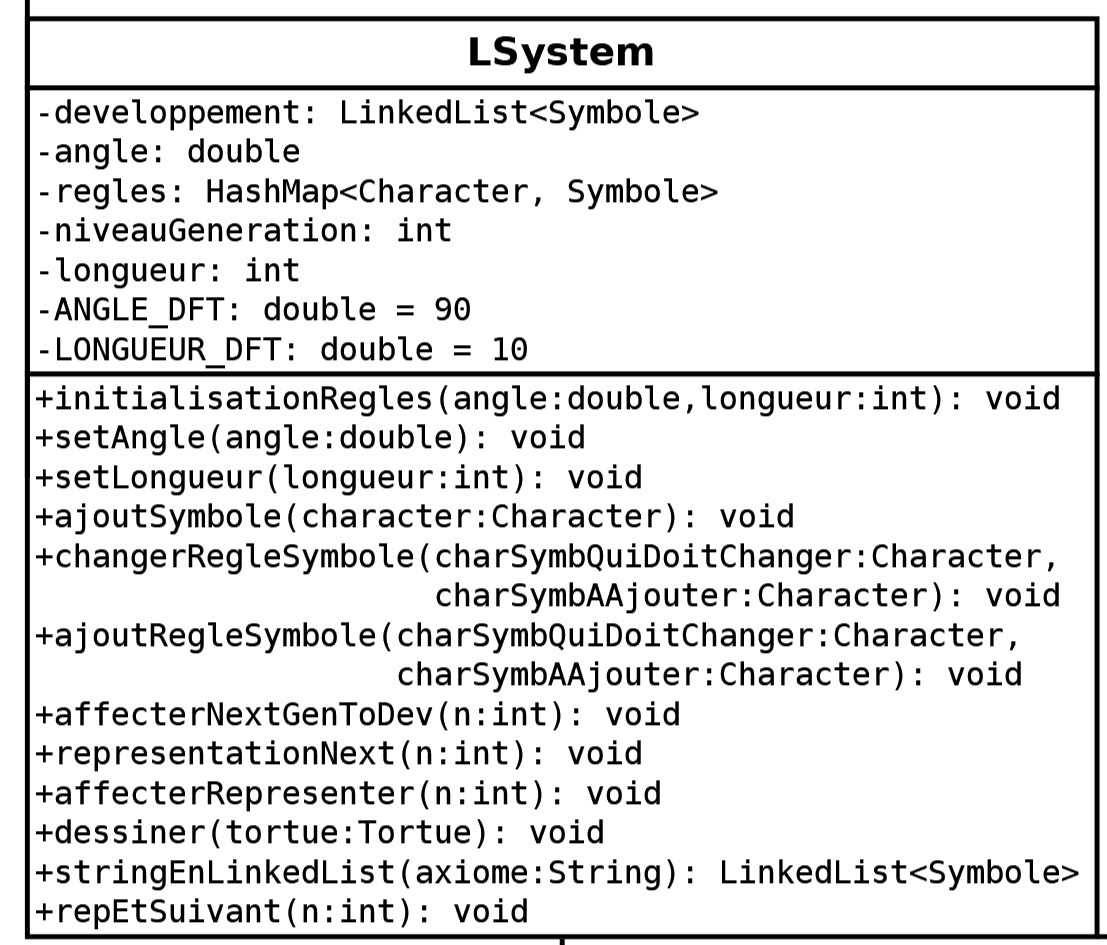
\includegraphics[width=\textwidth]{images/DiagrammeClasseLSystemOnly.png}
        \caption{Classe LSystem}
    \end{figure}
    \end{column}
    \end{columns}
\end{frame}
\subsection{Interface Graphique}
\begin{frame}{Interface Graphique}
    \begin{itemize}
        \item Interface au lancement
        \item Subdivision
        \item Interaction avec le L-Système \\ \begin{itemize}
            \item Gestion de la saisie
            \item Dessin de la tortue
        \end{itemize}
    \end{itemize}
\end{frame}
\begin{frame}{Interface au lancement}
    \begin{figure}[h]
	   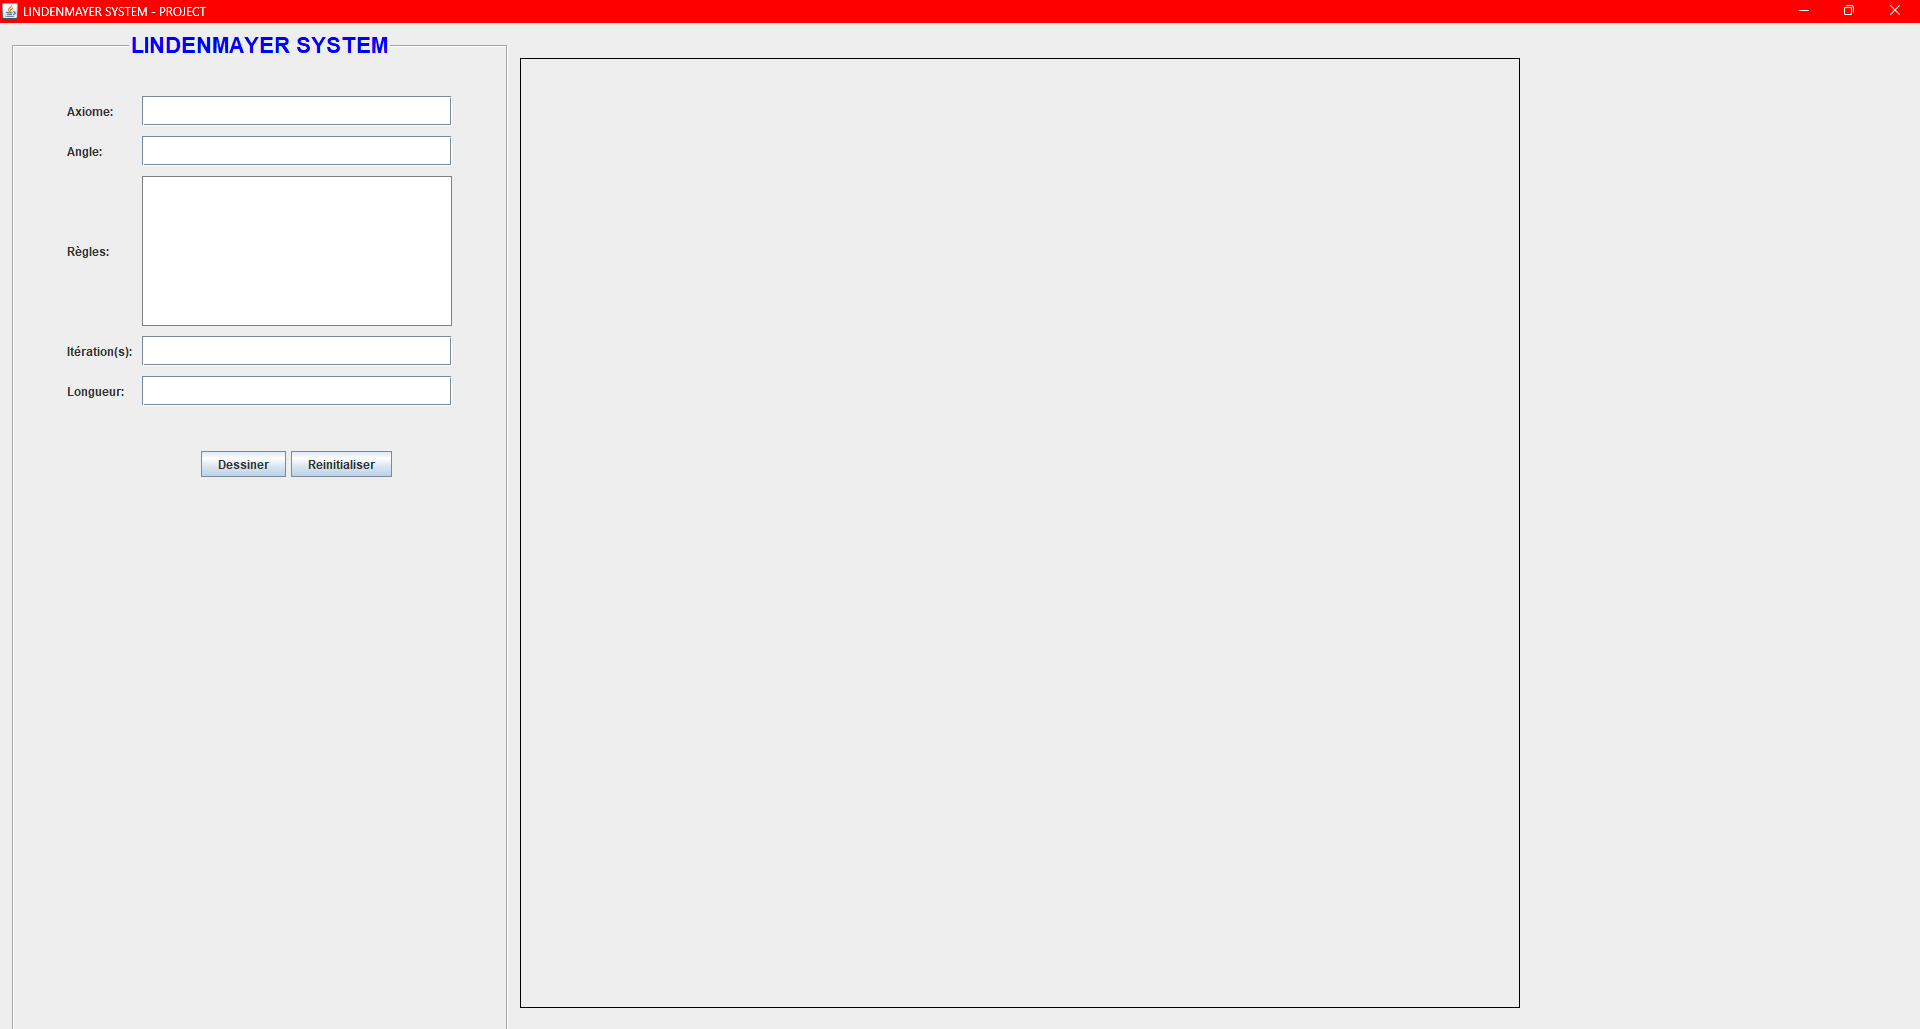
\includegraphics[width=\textwidth]{./images/LSystemVide.png}
	   \caption{LSytem vide}
    \end{figure}
\end{frame}
\section{Exemples}
\subsection{Quelques Résultats}
\begin{frame}{Quelques exemples}
    Voici quelques exemples de dessins générés :
    \begin{columns}[T]
        \begin{column}{0.5\textwidth}
            \begin{figure}
                \centering
                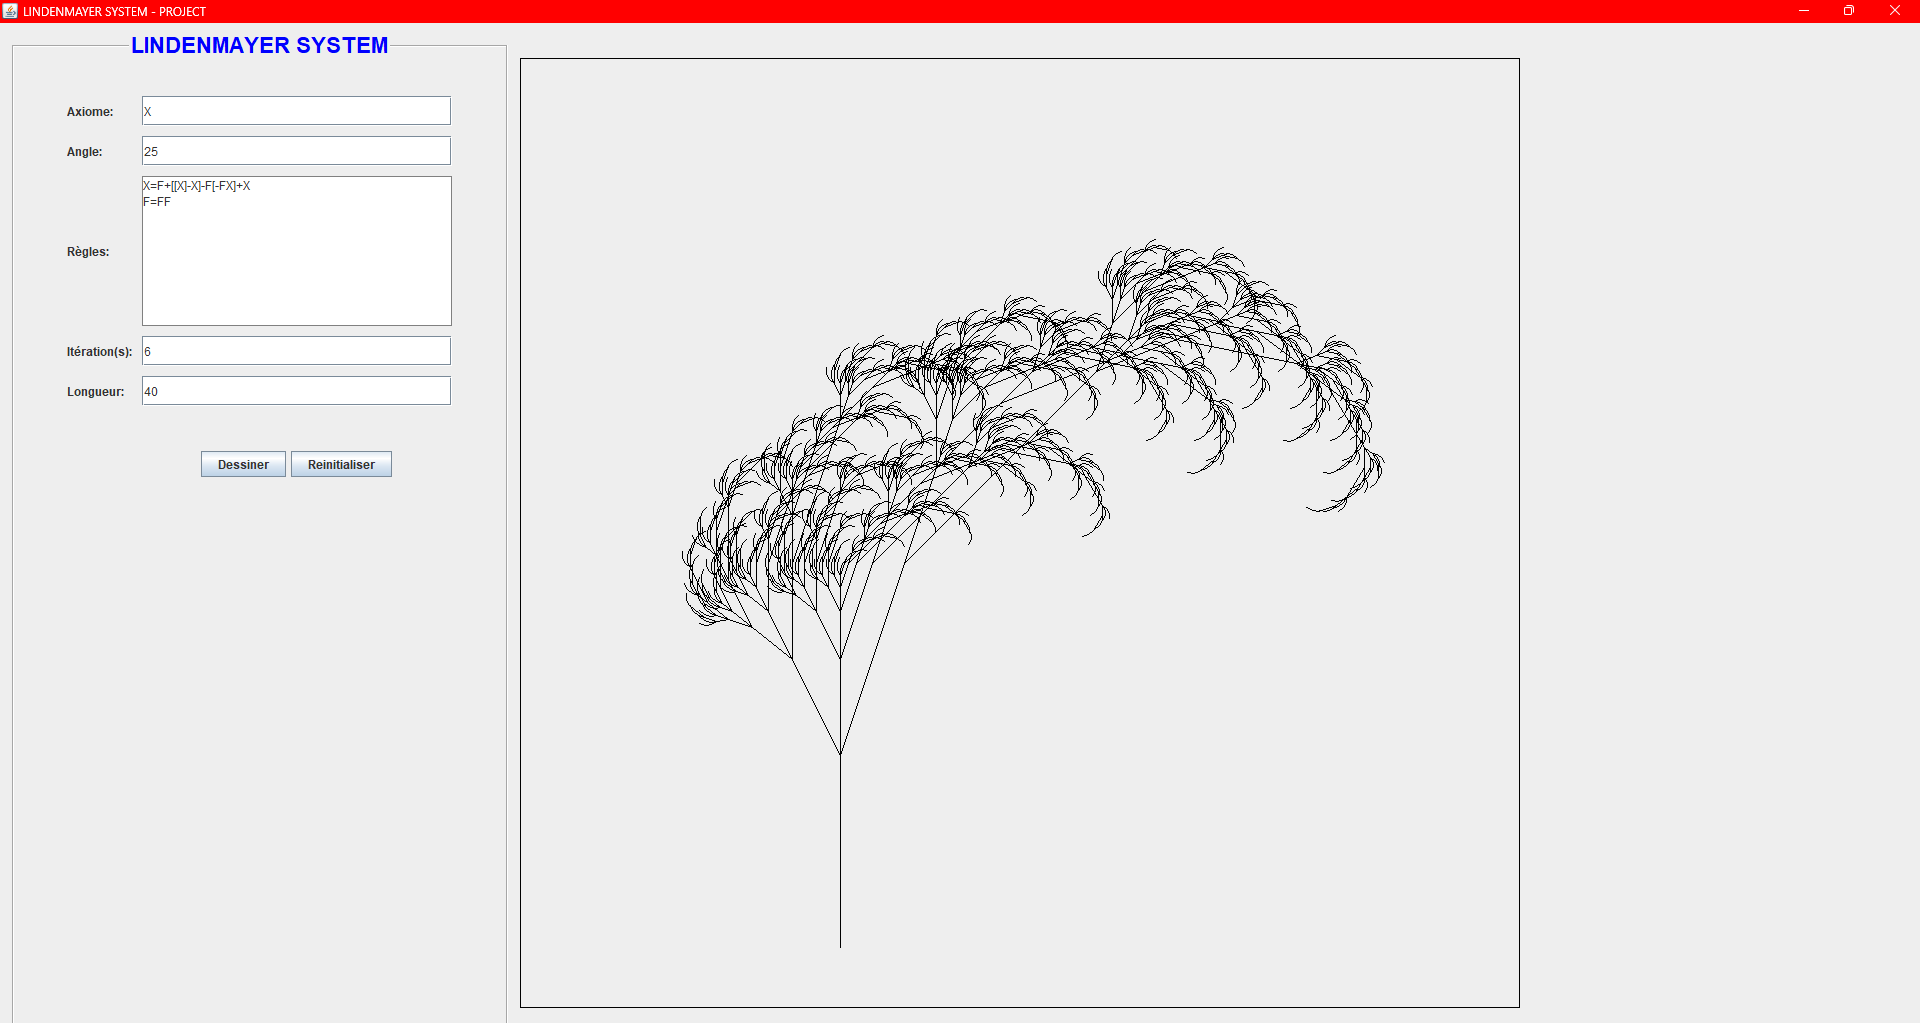
\includegraphics[width=0.75\textwidth]{./images/ArbreFractal.png}
                \caption{Arbre Fractal}
            \end{figure}
        \end{column}
            
        \begin{column}{0.5\textwidth}
            \begin{figure}
                \centering
                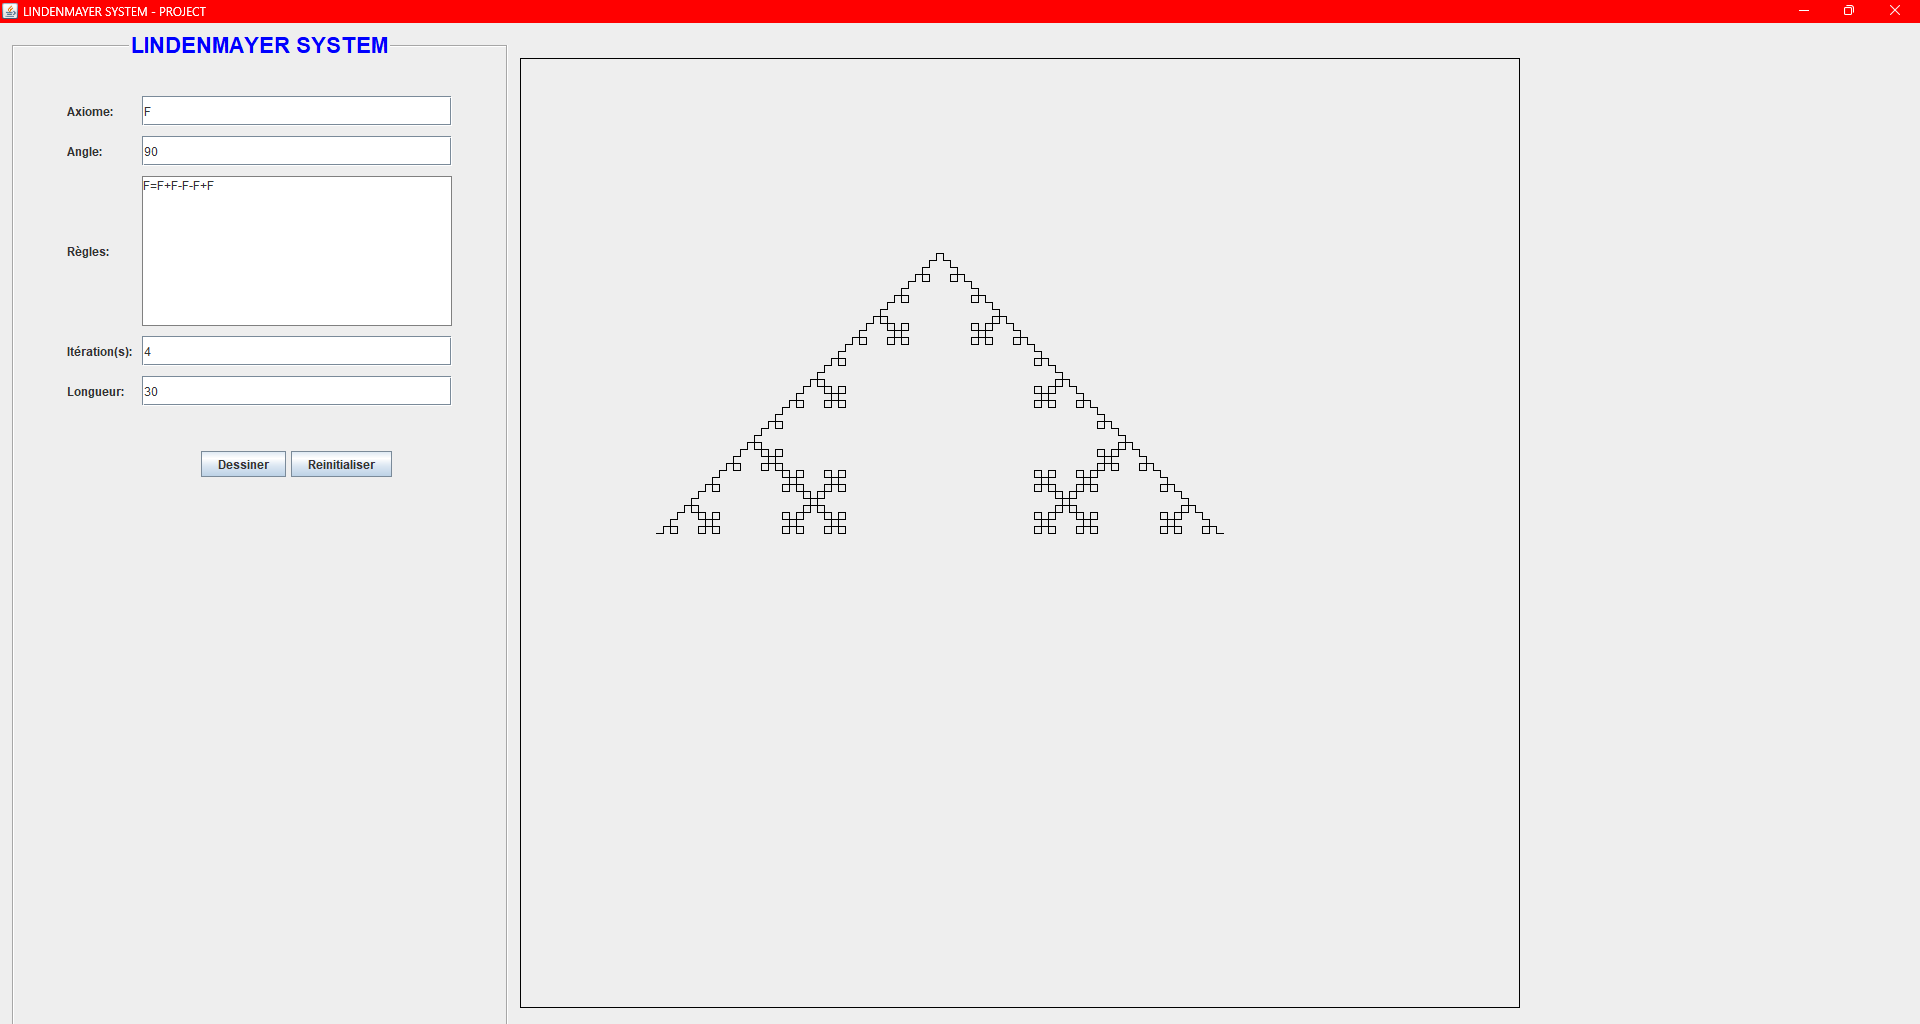
\includegraphics[width=0.75\textwidth]{./images/CourbeKoch.png}
                \caption{Courbe de Koch}
            \end{figure}
        \end{column}
    \end{columns}
    \begin{figure}
        \centering
        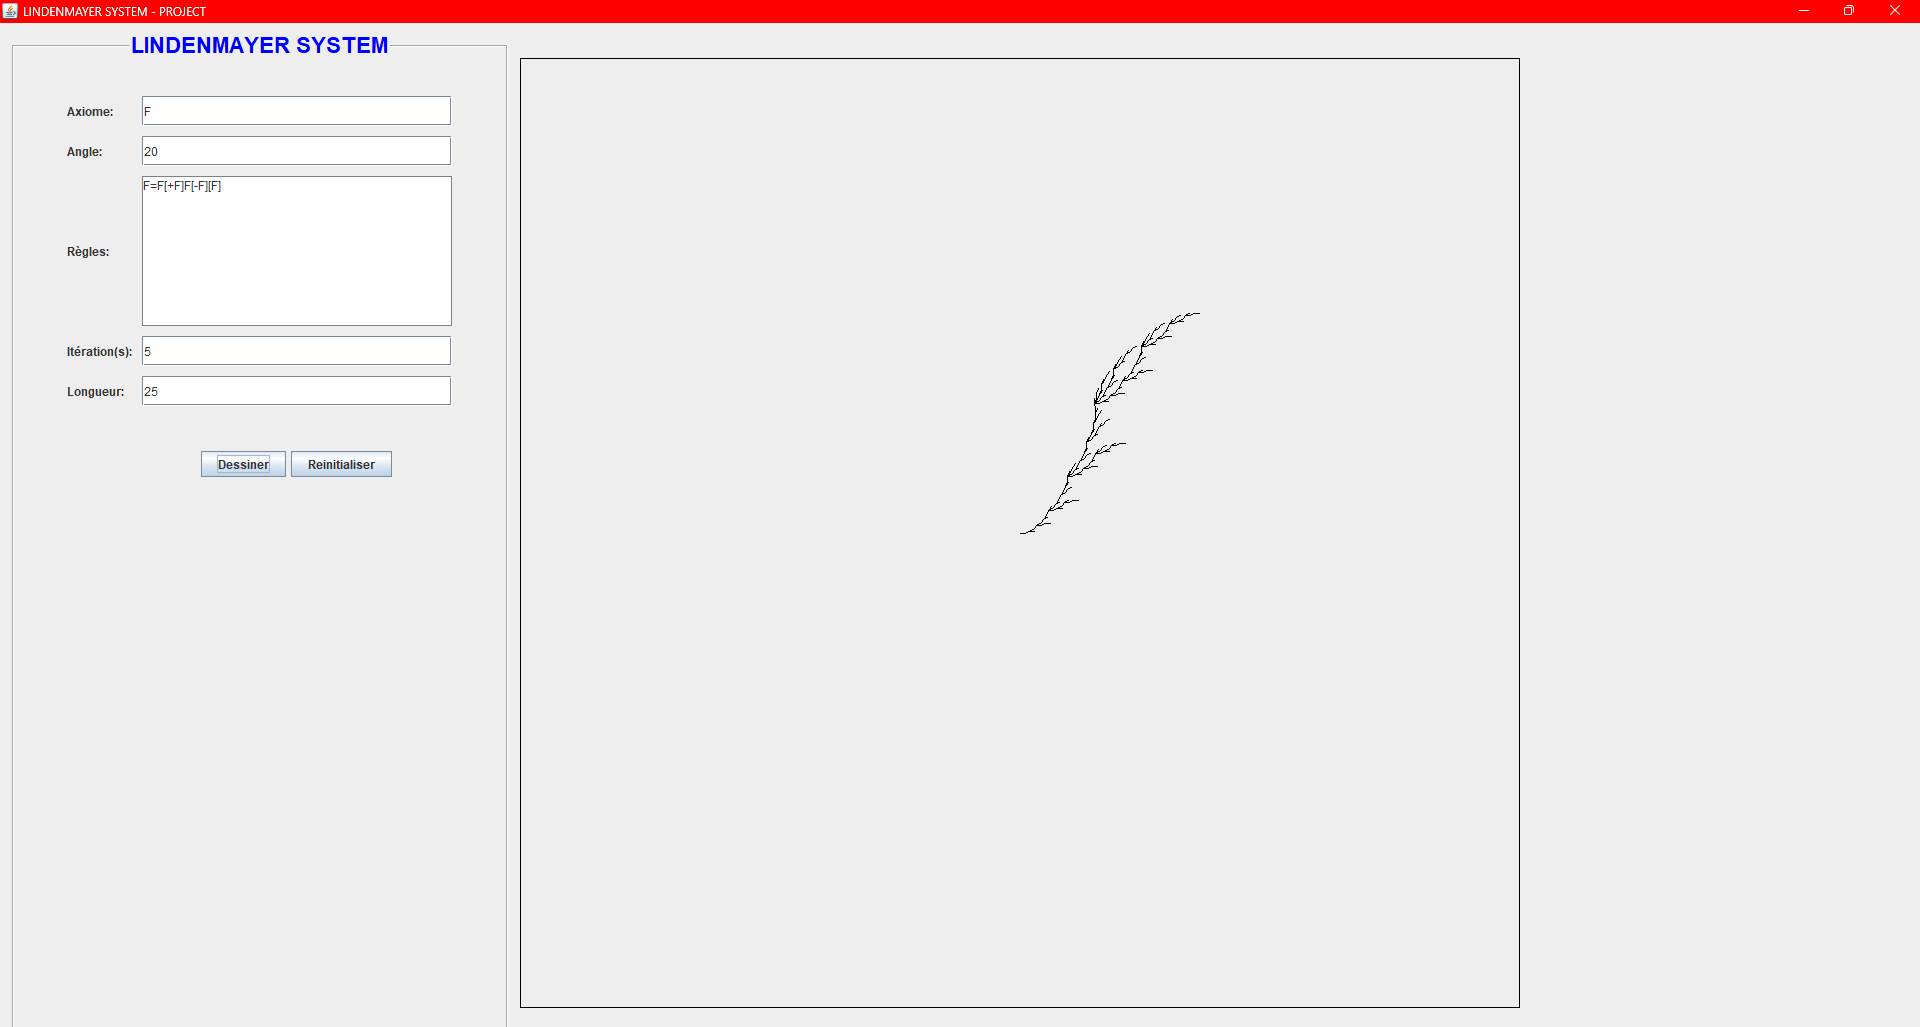
\includegraphics[width=0.35\textwidth]{./images/AutreArbre.png}
        \caption{Autre arbre fractal}
    \end{figure}
\end{frame}
\subsection{Démonstration}
\begin{frame}{Démonstration}
	Voici une vidéo de démonstration d'une génération d'arbre grâce à notre logiciel:
    \textbf{\textit{\href{run:video/demoLScuted.mp4}{video.mp4}}}
\end{frame}
\section{Conclusion}

\begin{frame}{Conclusion}
    \begin{itemize}
        \item Conclusion sur notre projet
        \item Propositions d'améliorations
    \end{itemize}
\end{frame}
\begin{frame}{Merci de votre attention accordée}
    Nous vous remercions de nous avoir écouter et accompagner tout le long.
\end{frame}


\end{document}